\documentclass[11pt]{article}

% Packages
\usepackage{amsmath}
\usepackage{graphicx}
\usepackage{amssymb}
\usepackage{longtable}
\usepackage[spanish]{babel}
\usepackage[utf8]{inputenc}
\usepackage[T1]{fontenc}
\usepackage{float}


\author{Brian Ameht Inclán Quesada C-411\\ Davier Sánchez Bello C-412\\ Eric López Tornas C-411}
\title{Proyecto Final de IA y Simulación \\ Juego de Supervivencia}
\date{}

% Document
\begin{document}

\maketitle
\newpage

\tableofcontents
\newpage

\section{Introducción}

\section{Modelo}
\subsection{Resumen del modelo}
\subsection{Ventajas}
\subsection{Desventajas}
\subsection{Posibles mejoras}


\section{Implementación}
\subsection{Modelo de la simulación}
\subsection{Agentes}
En nuestra simulación de supervivencia, utilizamos varios tipos de agentes, cada uno con estrategias y objetivos específicos que influyen en su comportamiento dentro del juego.Todos tienen un sistema experto que emula el conocimiento y la toma de decisiones del agente,
basandoce en la información que se le proporciona en el entorno de juego. Estas desiciones se toman en dependencia de las regls que se definan en el sistema experto, más explicado adelante. A continuación, describimos los tipos de agentes que utilizamos en nuestra simulación:

\subsubsection{Agente Aleatorio (RandomAgent)}
El \textit{RandomAgent} es un tipo de agente diseñado para tomar decisiones de manera aleatoria dentro de un entorno simulado. Este agente es una extensión de \textit{Agent\_with\_Memories}, lo que implica que puede recordar interacciones pasadas y datos del entorno para influir en sus decisiones futuras. Utiliza un sistema de estrategia basado en hechos y reglas para manejar su comportamiento en la simulación.

\paragraph{Funcionalidad del \textit{RandomAgent}}
\begin{itemize}
    \item \textbf{Inicialización}: Al crearse, se le asignan varios hechos iniciales como alianzas, enemigos, movimientos posibles, y recursos, entre otros. Estos hechos forman la base de su toma de decisiones.
    \item \textbf{Movimiento}: El agente decide su próximo movimiento de forma aleatoria entre los movimientos posibles disponibles, basándose en la estrategia actual.
    \item \textbf{Ataque}: Puede decidir atacar a otros agentes en su entorno si los ve. La decisión de atacar y la selección del objetivo son aleatorias, y el ataque se divide equitativamente entre los agentes visibles.
    \item \textbf{Asociaciones}: El agente puede recibir propuestas para unirse a asociaciones y decide aleatoriamente si unirse o no.
    \item \textbf{Interacción con el entorno}: Recibe y procesa información sobre objetos, recursos y acciones de otros agentes dentro de su entorno.
\end{itemize}

\paragraph{Reglas Definidas}
\begin{enumerate}
    \item \textbf{Regla de Movimiento (\textit{move\_rule})}:
          \begin{itemize}
              \item \textbf{Condición}: Se activa si hay movimientos posibles disponibles.
              \item \textbf{Acción}: Elige un movimiento aleatoriamente de los posibles y lo establece como el próximo movimiento.
          \end{itemize}
    \item \textbf{Regla de Ataque (\textit{attack\_rule})}:
          \begin{itemize}
              \item \textbf{Condición}: Se activa si hay otros agentes visibles en el entorno y decide aleatoriamente si realizar un ataque.
              \item \textbf{Acción}: Si decide atacar, distribuye los recursos de ataque disponibles equitativamente entre los agentes visibles y selecciona un subconjunto aleatorio de estos para atacar.
          \end{itemize}
\end{enumerate}

Estas reglas permiten al \textit{RandomAgent} operar en un entorno dinámico donde las decisiones no siguen un patrón predecible, lo que puede ser útil para simular comportamientos impredecibles o para probar la robustez de otros agentes dentro de la simulación.

\subsubsection{Agente Pacífico (PacifistAgent)}
El \textit{PacifistAgent} es un agente diseñado para evitar conflictos y minimizar las interacciones hostiles dentro de la simulación del juego de supervivencia. Este agente sigue una estrategia de no agresión, priorizando la evasión y la preservación por encima de la confrontación. A continuación, se describen sus funcionalidades y las reglas específicas que guían su comportamiento en el entorno simulado.

\paragraph{Funcionalidades del \textit{PacifistAgent}}
\begin{itemize}
    \item \textbf{Inicialización}: Al inicio, el agente configura hechos iniciales como alianzas, enemigos, y otros agentes en el entorno. Establece su memoria geográfica y de ataques, lo cual influye en su toma de decisiones estratégica.
    \item \textbf{Decisiones de Movimiento}: Basa sus movimientos en un conjunto de reglas evaluadas continuamente para elegir rutas que maximicen la distancia de las amenazas.
    \item \textbf{Reacción a Ataques}: Actualiza su conocimiento sobre enemigos y modifica su ruta al recibir ataques para mantenerse lo más distante posible del atacante.
    \item \textbf{Interacción Social}: Puede recibir propuestas de asociación y decide si participar basándose en su estrategia de no confrontación.
    \item \textbf{Observación del Entorno}: Continuamente actualiza su base de conocimientos con información sobre objetos y acciones observadas para tomar decisiones informadas.
\end{itemize}

\paragraph{Reglas del \textit{PacifistAgent}}
\begin{enumerate}
    \item \textbf{Regla para Moverse Lejos del Atacante (\textit{move\_away\_rule})}:
          \begin{itemize}
              \item \textbf{Condición}: Activada al recibir un ataque.
              \item \textbf{Acción}: Calcula y ejecuta un movimiento que incrementa la distancia entre él y el atacante.
          \end{itemize}
    \item \textbf{Regla para Observar Objetos (\textit{see\_objects\_rule})}:
          \begin{itemize}
              \item \textbf{Condición}: Activada cuando hay objetos visibles que pueden representar una amenaza.
              \item \textbf{Acción}: Evalúa y ajusta la ruta para evitar los objetos identificados como amenazas.
          \end{itemize}
    \item \textbf{Regla para Observar Acciones (\textit{see\_actions\_rule})}:
          \begin{itemize}
              \item \textbf{Condición}: Activada al observar acciones que pueden necesitar una respuesta evasiva.
              \item \textbf{Acción}: Analiza las acciones y decide la mejor ruta de evasión.
          \end{itemize}
    \item \textbf{Movimiento por Defecto (\textit{default\_move})}:
          \begin{itemize}
              \item \textbf{Condición}: Activada cuando no hay amenazas inmediatas detectadas.
              \item \textbf{Acción}: Selecciona un movimiento al azar de las opciones disponibles.
          \end{itemize}
\end{enumerate}

Estas reglas permiten al \textit{PacifistAgent} operar en un entorno dinámico y potencialmente hostil de manera que evita conflictos, lo cual es crucial para su supervivencia en el juego.

\subsubsection{Agente de Combate (CombatantAgent)}
El \textit{CombatantAgent} está diseñado para operar en entornos altamente hostiles y está enfocado en la confrontación directa. Utiliza estrategias complejas para maximizar su eficacia en el combate, respondiendo agresivamente a cualquier amenaza percibida.

\paragraph{Funcionalidades}
\begin{itemize}
    \item Inicializa con una configuración detallada de conocimientos que guiarán sus decisiones tácticas y estratégicas en el campo de batalla.
    \item Responde dinámicamente a los ataques, eligiendo la mejor acción basada en la evaluación continua del entorno.
    \item Observa y analiza constantemente el entorno para adaptar sus estrategias y movimientos.
\end{itemize}

\paragraph{Reglas Definidas}
\begin{enumerate}
    \item \textbf{Ataque a Enemigos Visibles}: Lanza ataques coordinados contra enemigos detectados dentro de su rango visual.
    \item \textbf{Movimiento Táctico}: Se mueve estratégicamente para posicionar mejor o evitar ataques.
    \item \textbf{Reacción a Ataques Recibidos}: Define la estrategia de respuesta, ya sea evasiva o de contraataque, basada en la naturaleza del ataque recibido.
    \item \textbf{Movimiento por Defecto}: Realiza un movimiento predeterminado cuando no hay decisiones claras de combate o movimiento.
\end{enumerate}

Estas reglas le permiten al \textit{CombatantAgent} manejar situaciones de combate con un enfoque estratégico y táctico, asegurando que cada acción tomada maximice su potencial de supervivencia y éxito en el combate.

\subsubsection{Agente Inteligente (SmartAgent)}
El \textit{SmartAgent} utiliza algoritmos avanzados de toma de decisiones y aprendizaje automático para adaptar su comportamiento basado en la dinámica del juego. Este agente evalúa constantemente el estado del juego, tomando decisiones informadas sobre cuándo recolectar recursos, combatir, o retirarse basado en las probabilidades de éxito y supervivencia.

\subsubsection{Agente Buscador de Comida (FoodSeekerAgent)}
El \textit{FoodSeekerAgent} es un agente programado para enfocarse intensamente en la localización y recolección de recursos alimenticios dentro de la simulación. Evita el combate en la medida de lo posible, priorizando la acumulación de recursos para garantizar su supervivencia.

\paragraph{Funcionalidades}
\begin{itemize}
    \item Configura hechos iniciales que incluyen la memoria geográfica y táctica, cruciales para la navegación y las decisiones estratégicas.
    \item Se especializa en la eficiente localización y consumo de recursos, utilizando avanzados algoritmos de búsqueda para optimizar sus rutas.
    \item Prefiere evitar conflictos, eligiendo caminos que minimicen el contacto con otros agentes agresivos.
\end{itemize}

\paragraph{Reglas Definidas}
\begin{enumerate}
    \item \textbf{Comer sin Enemigos}: Optimiza el movimiento hacia los recursos cuando no hay amenazas cercanas.
    \item \textbf{Comer con Enemigos}: Decide entre aprovechar los recursos o moverse a una posición más segura si hay enemigos cerca.
    \item \textbf{Movimiento por Defecto}: Realiza un movimiento estándar cuando no se detectan recursos o amenazas inmediatas.
    \item \textbf{Situaciones de Atasco y Recursos Disponibles}: Resuelve bloqueos en su ruta para continuar hacia los recursos.
\end{enumerate}

Estas reglas permiten al \textit{FoodSeekerAgent} operar eficazmente en un entorno donde la obtención de recursos es crucial para la supervivencia.

\subsection{Base de conocimiento y toma de decisiones}
Este sistema se basa en una estructura modular que integra hechos y reglas dentro de un motor de inferencia para gestionar y tomar decisiones basado en conocimientos. Está diseñado para funcionar en entornos donde las decisiones se toman a partir de un conjunto de datos dinámico y posiblemente en tiempo real. Los componentes clave son:

\begin{itemize}
    \item \textbf{Enumeración \textit{Knowledge}:} Es una enumeración que define diferentes tipos de conocimientos que pueden ser importantes en un contexto de toma de decisiones. Estos incluyen aspectos como la posición, la salud, los ataques disponibles, las asociaciones y más. Cada tipo de conocimiento sirve como una clave que identifica un tipo de información específica dentro del sistema
    \item \textbf{Clase \textit{Fact}:}  Representa un hecho o una pieza de información en el sistema. Cada hecho está compuesto por una clave (un valor de Knowledge) y un dato asociado a esta clave. Esta estructura permite almacenar y gestionar información dinámica que el sistema utiliza para tomar decisiones
    \item \textbf{Clase \textit{Rule}:}  Define una regla en el sistema, la cual consta de una condición y una acción. La condición es una función que toma un conjunto de hechos y determina si la regla debe ejecutarse. Si la condición es verdadera, la acción (también una función) se ejecuta para generar nuevos hechos basados en los hechos existentes. En resumen, esta clase permite definir la lógica del sistema para generar nuevos hechos a partir de los existentes.
    \item \textbf{Clase \textit{BaseKnowledge}:} Esta clase especifica las operaciones fundamentales para cualquier sistema de conocimiento, como aprender y tomar decisiones.
    \item \textbf{Clase \textit{Estrategy}:} Es una implementación concreta de BaseKnowledge. Gestiona un conjunto de hechos y reglas a través de un motor de inferencia. Permite añadir y eliminar conocimientos y reglas, aprender de nuevos datos y tomar decisiones basadas en las reglas definidas y los hechos actuales
    \item \textbf{Clase \textit{InferenceEngine}:} Es el componente que realiza la inferencia lógica. Gestiona un conjunto de hechos y reglas, permitiendo añadir y eliminar estos elementos. El método run de InferenceEngine es crucial: evalúa todas las reglas con los hechos actuales para generar nuevos hechos, los cuales pueden influir en decisiones futuras.
\end{itemize}

Este modelo permite un manejo flexible y dinámico de información, esencial para la toma de decisiones en entornos cambiantes, tal y como necesitamos en nuestra simulacion.
\subsection{Algoritmos de búsqueda}
En esta sección, describiremos varios algoritmos de búsqueda utilizados en nuestro proyecto. Cada algoritmo será tratado en una subsección independiente, donde se explicará su funcionamiento, particularidades y ejemplos de uso.

\subsubsection{Algoritmo A*}
El algoritmo A* es una técnica de búsqueda de camino que encuentra el camino más corto entre un nodo inicial y un nodo objetivo en un grafo. Utiliza una combinación de costos conocidos para llegar a un nodo \( g(n) \) y una estimación heurística \( h(n) \) del costo para alcanzar el objetivo desde ese nodo. La función \( f(n) = g(n) + h(n) \) guía el algoritmo para explorar los caminos más prometedores primero.

En nuestro caso estamos implementado usando una estructura de tipo $min-heap$, denominada $open\_heap$. Esta estructura se utiliza para mantener los nodos que aún necesitan ser explorados en el algoritmo. Mediante un heap de minimos organiza los elementos de tal manera que el primer elemento es siempre el más pequeño, lo cual es útil para extraer rápidamente el nodo con el costo estimado más bajo para continuar la búsqueda.


\paragraph{Detalles del Funcionamiento}
\begin{itemize}
    \item \textbf{Heurística}: La función heurística es crucial en A*. Una elección común es la distancia Manhattan, útil en grillas donde solo se permiten movimientos horizontales y verticales.
    \item \textbf{Conjunto de abiertos}: A* mantiene un conjunto de nodos conocidos como el "conjunto abierto". Inicialmente, contiene solo el nodo de inicio.
    \item \textbf{Bucle Principal}: En cada paso del algoritmo, el nodo con el menor valor de \( f(n) \) se retira del conjunto abierto. Este nodo es procesado considerando todos sus nodos vecinos. Para cada vecino, se calcula \( g(n) \) y \( h(n) \), y si el nuevo camino es mejor, se actualiza el camino.
\end{itemize}

\paragraph{Ejemplo de Uso}
En el siguiente ejemplo mostramos un agente del tipo $FoodSeekerAgent$ que en nuestra simulacion representa al agente que esta constantemente buscando la mejor manera de llegar al lugar donde mas recursoa halla. En este caso tenemos un tablero de \(10 \times 10\). Definimos la posición inicial como \( (0, 8) \) y el objetivo en este caso la casilla que dentro de su rango de vision
es la que mas recursos posee, como \( (2, 9) \). La salida del algoritmo proporcionará la secuencia de movimientos para llegar del inicio al objetivo, evitando los obstáculos, que en este ejemplo no hay ninguno.

\begin{figure}[H]
    \centering
    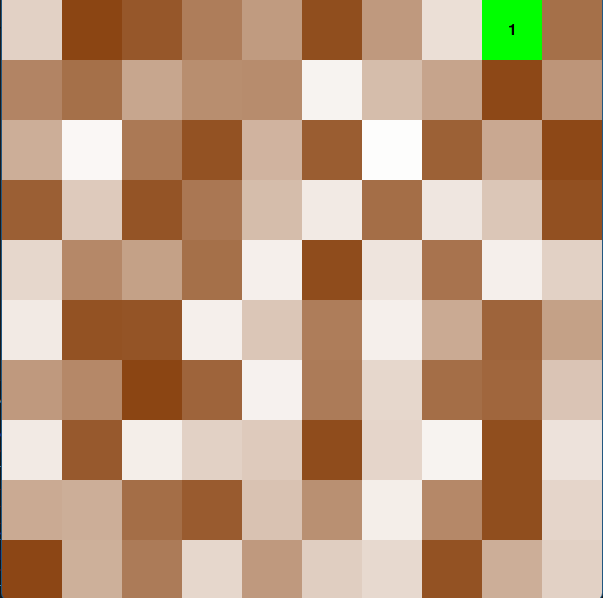
\includegraphics[width=0.18\textwidth]{images/image1.png}\hfill
    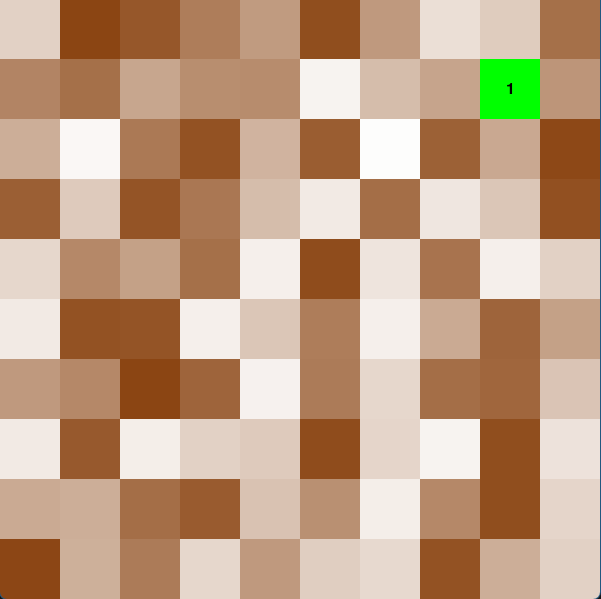
\includegraphics[width=0.18\textwidth]{images/image2.png}\hfill
    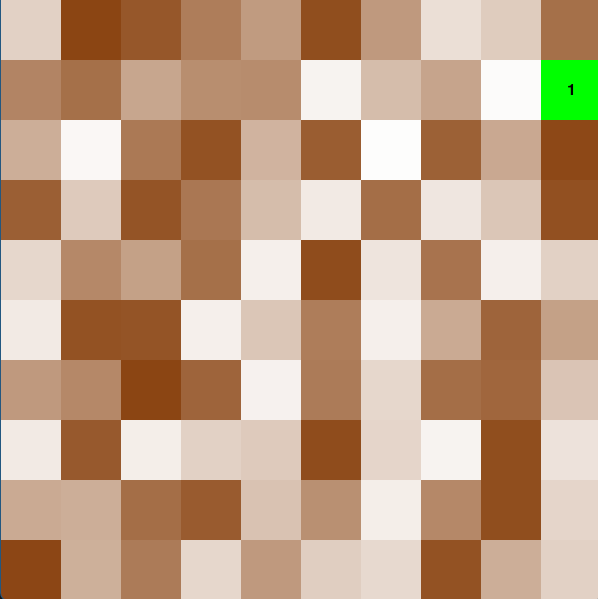
\includegraphics[width=0.18\textwidth]{images/image3.png}\hfill
    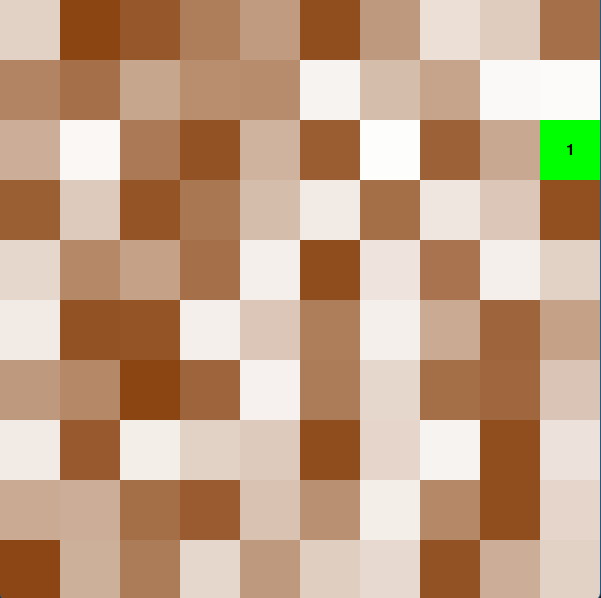
\includegraphics[width=0.18\textwidth]{images/image4.png}
    \caption{Secuencia de movimientos del agente FoodSeekerAgent en la simulación desde la posicion \( (0, 8) \) hasta \( (2, 9) \) .}
\end{figure}

\paragraph{Implementación}
Para implementar el A* en la simulación de nuestro juego, utilizamos una clase que gestiona la verificación de movimientos válidos y obstáculos. Esta clase ajusta el algoritmo para adaptarse a las características específicas del entorno de juego, como áreas inaccesibles y diferentes costos de movimiento asociados con diversos tipos de terreno.

\subsubsection{Búsqueda en Amplitud (BFS)}
La Búsqueda en Amplitud, o BFS por sus siglas en inglés (Breadth-First Search), es un algoritmo clásico para explorar grafos y árboles. Es especialmente útil en situaciones donde necesitamos encontrar el camino más corto en términos de número de aristas entre un nodo de origen y otros nodos, dado que explora todos los nodos a la misma profundidad antes de moverse a la profundidad siguiente.
En nuestra simulación está especialmente diseñado para calcular rutas de escape en situaciones donde un agente necesita maximizar la distancia de un atacante en un entorno de grilla. La adaptación permite a los usuarios elegir entre obtener sólo el siguiente movimiento óptimo o el camino completo de escape.

\paragraph{Funcionamiento de BFS}
La implementación de BFS comienza con la inserción del nodo de origen en una cola. A medida que cada nodo se procesa, sus vecinos no visitados se añaden al final de la cola. Este proceso continúa hasta que se visitan todos los nodos alcanzables o hasta que se encuentra el nodo objetivo, lo que permite una exploración completa en capas.

\begin{itemize}
    \item \textbf{Cola de BFS}: Utilizamos una cola para mantener el orden de exploración de los nodos. En nuestra implementación, esto se maneja con una estructura de datos deque para una eficiente inserción y eliminación de elementos.
    \item \textbf{Conjunto de Obstáculos y Visitados}: Mantenemos un conjunto de obstáculos para evitar la exploración de nodos no transitables y un conjunto de nodos visitados para evitar procesar el mismo nodo más de una vez.
    \item \textbf{Validación de Movimientos}: Cada movimiento potencial se valida para asegurar que no se salga del límite del entorno de juego y no se encuentre con obstáculos.
\end{itemize}

\paragraph{Ejemplo de Uso}
En el siguiente ejemplo, mostramos un agente del tipo $PacifistAgent$ \( (azul) \) en la posicion \( (5, 6) \), que en nuestra simulación representa al agente que tiene una estrategia pacifica, evade los ataques e intenta sobrevivir.
En este caso, tenemos un tablero de \(7 \times 7\). Definimos la posición inicial del agente $CombatantAgent$ \( (rojo) \) como \( (3, 3) \). La salida del algoritmo proporcionará la secuencia de movimientos para llegar a la posición segura más lejana posible, evitando al atacante, evidenciamos en las siguientes imagenes como
la secuencia de movimientos incluye como primer movimiento el de alejarce del atacante hacia la casilla \( (6, 6) \), luego en el siguiente movimiento, este se queda en esa misma posicion ya que de entre las posibles es la mas lejana al atacante


\begin{figure}[H]
    \centering
    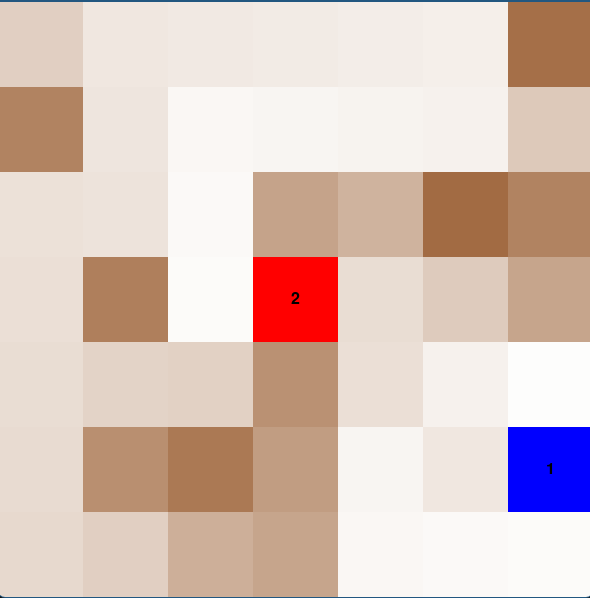
\includegraphics[width=0.18\textwidth]{images/image6.png}\hfill
    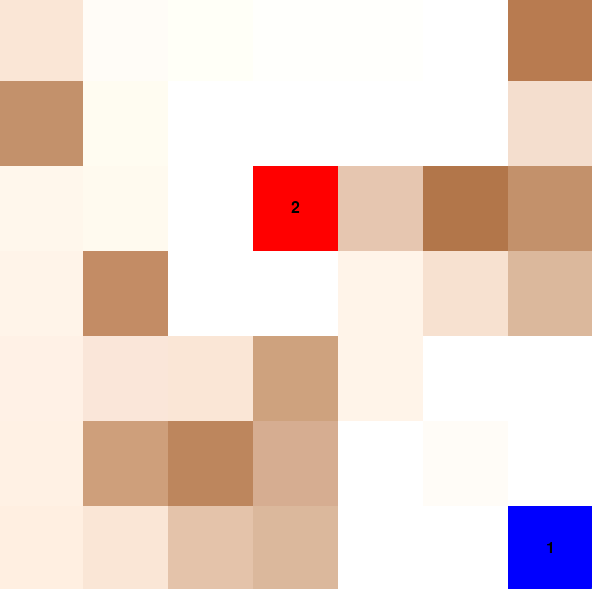
\includegraphics[width=0.18\textwidth]{images/image7.png}\hfill
    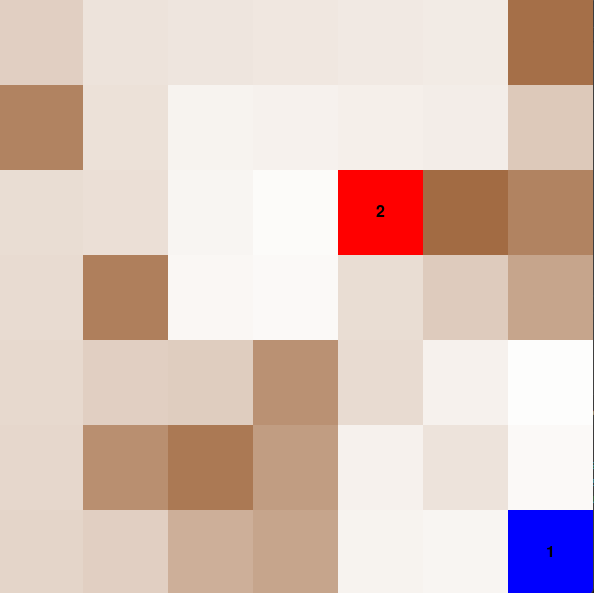
\includegraphics[width=0.18\textwidth]{images/image8.png}
    \caption{Secuencia de movimientos calculada por BFS para evadir al atacante, mostrando cada paso desde el inicio hasta la posición segura más lejana posible.}
\end{figure}

\paragraph{Implementación}
Nuestra clase \textit{BFS} incluye métodos para configurar los obstáculos y calcular la ruta basada en las posiciones dinámicas de los agentes y las barreras en el entorno. Esto asegura que el agente siempre tenga una ruta de escape actualizada y pueda reaccionar a los cambios en el entorno.



\subsubsection{Monte Carlo Tree Search (MCTS)}
El Monte Carlo Tree Search es un algoritmo de búsqueda heurística utilizado para la toma de decisiones en juegos de perfecta información. Combina la exploración aleatoria de árboles con la simulación para evaluar los movimientos potenciales.

\paragraph{Funcionamiento y Ejemplos}
Descripción del funcionamiento y ejemplos...



\subsection{LLM}
Utilizamos el LLM para la creación de agentes y la configuración del escenario de la simulación, así como para la función de comentarista del juego. Para la creación de agentes, empleamos una lista con descripciones por defecto de los comportamientos de nuestros tipos de personajes y la información suministrada por el usuario. El LLM infiere cuál es el tipo de personaje por defecto que más se acerca a la descripción del usuario, así como las estadísticas, teniendo en cuenta la mención u omisión de aspectos positivos y negativos en la descripción del personaje.
\\
En cuanto a la creación del mapa, se eligen las dimensiones del escenario a simular de acuerdo a la inferencia realizada por el LLM en la descripción del terreno.  \\
Para la función de comentarista, alimentamos al LLM con las últimas acciones ocurridas en la simulación y las descripciones de los personajes. Esto permite al modelo crear un breve relato de los eventos más recientes no comentados en la simulación.
\subsection{Interfaz de la simulación}

\section{Análisis de la simulación}
\section{Conclusiones}

\end{document}
